%%%%%%%%%%%%%%%%%%%%%%%%%%%%%%%%%%%%%%%%%
% University Assignment Title Page 
% LaTeX Template
% Version 1.0 (27/12/12)
%
% This template has been downloaded from:
% http://www.LaTeXTemplates.com
%
% Original author:
% WikiBooks (http://en.wikibooks.org/wiki/LaTeX/Title_Creation)
%
% License:
% CC BY-NC-SA 3.0 (http://creativecommons.org/licenses/by-nc-sa/3.0/)
% 
% Instructions for using this template:
% This title page is capable of being compiled as is. This is not useful for 
% including it in another document. To do this, you have two options: 
%
% 1) Copy/paste everything between \begin{document} and \end{document} 
% starting at \begin{titlepage} and paste this into another LaTeX file where you 
% want your title page.
% OR
% 2) Remove everything outside the \begin{titlepage} and \end{titlepage} and 
% move this file to the same directory as the LaTeX file you wish to add it to. 
% Then add \input{./title_page_1.tex} to your LaTeX file where you want your
% title page.
%
%%%%%%%%%%%%%%%%%%%%%%%%%%%%%%%%%%%%%%%%%
%\title{Title page with logo}
%----------------------------------------------------------------------------------------
%	PACKAGES AND OTHER DOCUMENT CONFIGURATIONS
%----------------------------------------------------------------------------------------

\documentclass[12pt]{article}
\usepackage[english]{babel}
\usepackage[utf8x]{inputenc}
\usepackage{amsmath}
\usepackage{graphicx}
\usepackage[colorinlistoftodos]{todonotes}

\usepackage{cite}
\usepackage{algorithmic}
\usepackage{textcomp}
\usepackage{xcolor}
\usepackage{subcaption}
\usepackage{url}
\usepackage{hyperref}



\textheight=250truemm \textwidth=138truemm 
\hoffset=-10truemm \voffset=-30truemm

\begin{document}

\begin{titlepage}

\newcommand{\HRule}{\rule{\linewidth}{0.5mm}} % Defines a new command for the horizontal lines, change thickness here

\center % Center everything on the page
 
%----------------------------------------------------------------------------------------
%	HEADING SECTIONS
%----------------------------------------------------------------------------------------

\textsc{\LARGE Ukrainian Catholic University}\\[1cm] % Name of your university/college
\textsc{\Large  Faculty of Applied Sciences}\\[0.5cm] % Major heading such as course name
\textsc{\large Data Science Master Programme}\\[0.5cm] % Minor heading such as course title

%----------------------------------------------------------------------------------------
%	TITLE SECTION
%----------------------------------------------------------------------------------------
\vspace*{1cm}

\HRule \\[0.4cm]
{ \huge \bfseries A Comparative Analysis of Linear Algebra Methods for Efficient Transformer Attention in Image Classification}\\[10pt]
{\Large \bfseries Linear Algebra final project report}\\[0.4cm] % Title of your document
\HRule \\[0.8cm]
 
%----------------------------------------------------------------------------------------
%	AUTHOR SECTION
%----------------------------------------------------------------------------------------
\vspace*{0.5cm}

% If you don't want a supervisor, uncomment the two lines below and remove the section above
\Large \emph{Authors:}\\
Anton \textsc{Brazhnyi}\\Olexandr \textsc{Korniienko}\\Andrii \textsc{Ruda}\\[1cm] % Your name

%----------------------------------------------------------------------------------------
%	DATE SECTION
%----------------------------------------------------------------------------------------
\vspace*{1cm}
{\large 28 February 2023}\\[2cm] % Date, change the \today to a set date if you want to be precise

%----------------------------------------------------------------------------------------
%	LOGO SECTION
%----------------------------------------------------------------------------------------


\includegraphics[height=5cm]{UCU-Apps.png}\\[1cm] % Include a department/university logo - this will require the graphicx package
 
%----------------------------------------------------------------------------------------

\vfill % Fill the rest of the page with whitespace

\end{titlepage}

\begin{abstract}
Attention is a critical component of transformer models, but its computational complexity limits its scalability. This project investigates linear algebra-based approaches to optimise the attention mechanism's performance, including low-rank approximations, kernels/factorisation, and other methods. We provide a detailed analysis of the computational complexity and compare their empirical performance on an image classification task.
\end{abstract}

\section{Introduction}
The Transformer architecture has become a cornerstone in modern deep learning and has led to numerous breakthroughs in natural language processing, computer vision, and other areas. The Transformer's attention mechanism has been shown to be a crucial component in its success. However, computing the attention scores for all pairs of positions in an input sequence results in quadratic time and memory complexity with respect to the sequence length, making the mechanism slow and memory-intensive for long input sequences.

In this project, we explore various methods for optimising the attention mechanism in the Transformer architecture. We focus on five methods: 
\begin{enumerate}
\item Full Attention
\item Linear Attention
\item Linformer Attention
\item Random Feature Attention
\item Nystrom Attention
\end{enumerate}
Each method uses linear algebra techniques to optimise the attention mechanism and reduce the computational and memory costs of the Transformer architecture. We will provide an overview of each method and compare their computational complexities and performance on an image classification task.


\section{Quick methods overview}

\subsection{Full Attention}

Attention calculates a weighted average of the feature representation with weight proportional to the similarity score between pairs of representations. Let’s consider input $X^{n \times d}$ and $W_q \in R^{d \times d_q}$, $W_k \in R^{d \times d_k}$, $W_v \in R^{d \times d_v}$ referred as query, key, and value projectors for input sequence with $n$ length. The projections (outputs) are then computed as $Q=XW_q$, $K=XW_k$, $V=XW_v$.
The attention layer is defined as 

$$ \text{Attention}(Q, K, V) = \text{Softmax} \big( \frac{QK^T}{\sqrt{d_k}} \big)V $$ 

which requires $O(n^2d)$ steps to compute and scales poorly with the large input size. An intuitive illustration of the Attention layer is presented in the figure \ref{fig:self-attention} below.

\begin{figure}[h]
\centering
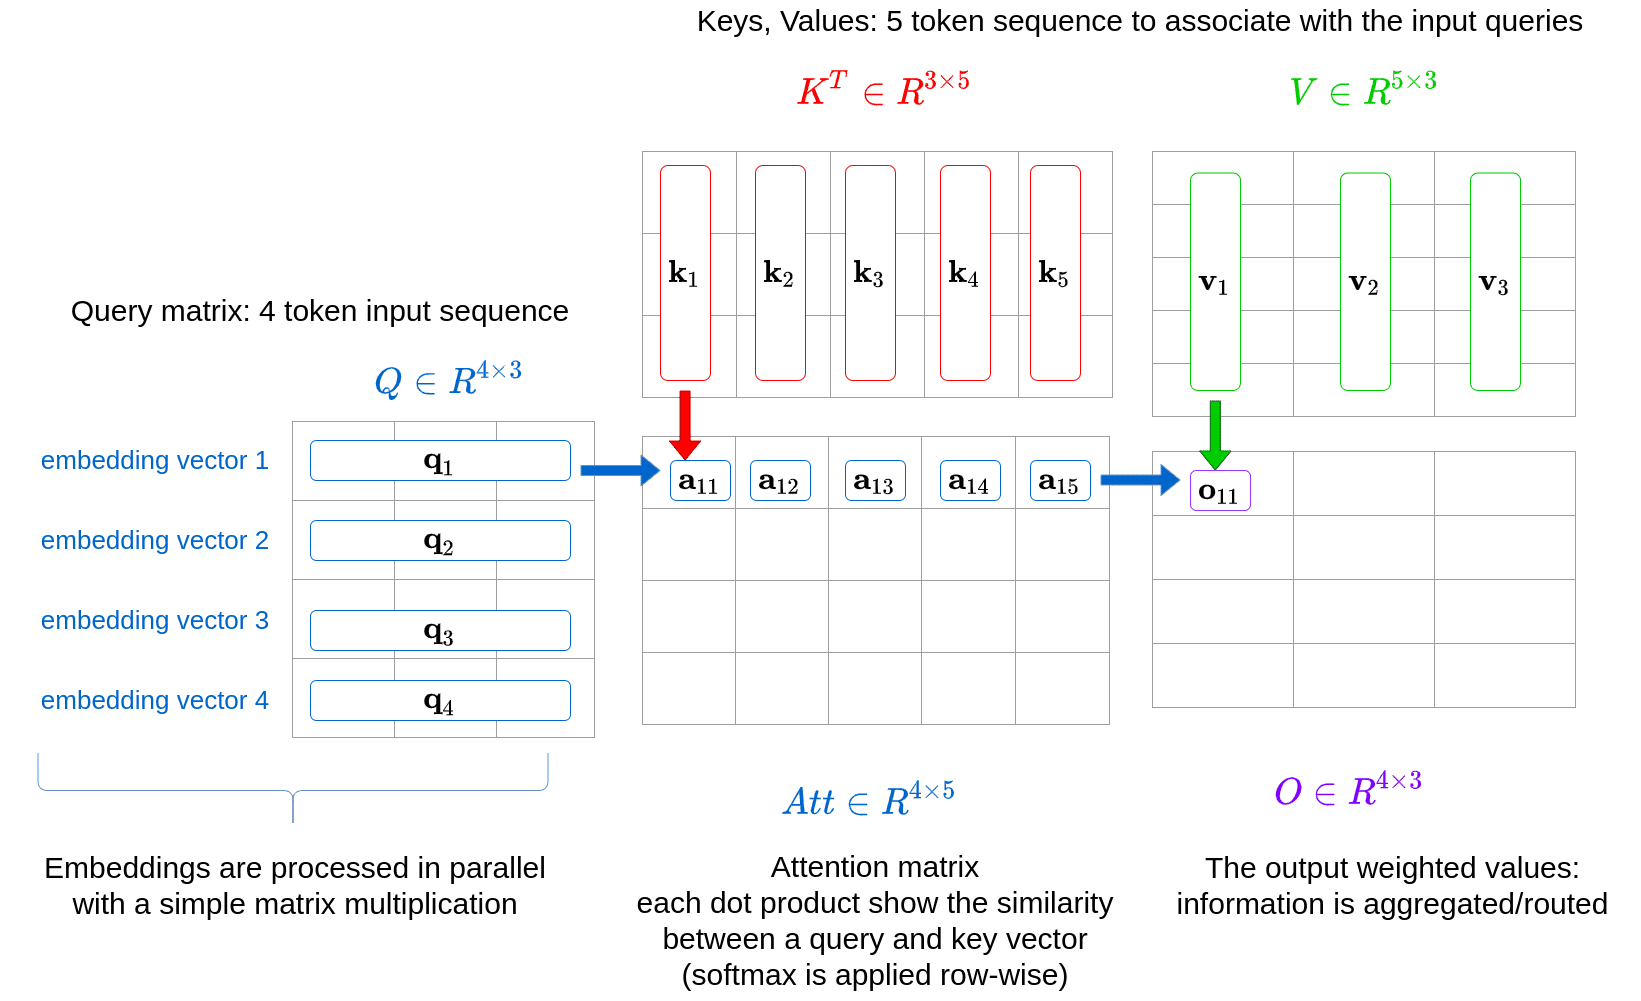
\includegraphics[width=0.5\textwidth]{self-attention-explained.png}
\caption{\label{fig:self-attention}Illustration of self-attention mechanism \cite{self-attention-explained}.}
\end{figure}

However, the scaled dot-product attention isn't simply applied to the queries, keys and values. Instead of this, single attention components with: queries, keys and values are splited into $ h $ heads and the scaled dot-product attention is calculated over all heads in parallel.

$$ \text{MultiHead}(Q, K, V) = \text{Concat}(\text{head}_1,...,\text{head}_h)W^O $$

$$ \text{head}^i = \text{Attention}(QW_q^i, KW_k^i, VW_v^i) $$

The standard attention mechanism used in the Transformer architecture computes attention scores for all pairs of positions in the input sequence, resulting in quadratic time and memory complexity.


\subsection{Linear Attention}

Dot-product attention has wide applications, but as we described in the previous section, its memory and computational costs grow quadratically with the input size. Such growth prohibits its application on high-resolution inputs. For this purpose, the efficient attention mechanism equivalent to dot-product attention is used. The Linear Attention mechanism allows for reducing memory and computational costs to remedy this drawback. At the same time, empirical evaluations \cite{linear-attention-transformer} demonstrated the effectiveness of its advantages.

Efficient attention proposes the individual feature vectors $ X \in R^{n \times d} $ still pass through three linear layers to form the queries Q keys K, and values V. However, instead of interpreting the keys as $n$ feature vectors in $R^{d_k}$, the module regards them as $d_k$ single-channel feature maps. Efficient attention uses each feature map as an overall weighting position and aggregates the value features through weighted summation to form a global context vector \cite{efficient-linear-attention}. 

The equation describes linear attention presented below:

$$ \text{Linear Attention}(Q, K, V) = \text{Softmax}_{row} \big(Q)\big ( \text{Softmax}_{col} \big( K \big)^T V) $$ 

To prove equivalence of the considered method to dot-product attention, let's replace Softmax normalizing function to $1 / \sqrt{d}$, so the original formula takes a form:
$$ \text{Attention}(Q, K, V) = \big( \frac{QK^T}{d_k} \big)V $$ 

Linear attention can be expressed in the following way
$$ \text{Linear Attention}(Q, K, V) =  \big( \frac{Q}{\sqrt(d_k)} \big) \big( \frac{K^T}{\sqrt(d_k)} V ) = \frac{1}{d_k} Q \big( K^T V \big) = \frac{1}{d_k} \big(Q K^T\big) V = \text{Attention}(Q, K, V)$$ 

The main advantages of the algorithms are:

\begin{itemize}
\item improved computational complexity from $ O(d * n^2) $ (for dot-product attention) to $ O(d^2 * n) $ for linear attention
\item increase memory efficiency from  $ O(n^2) $ to  $ O(dn+d^2) $ respectively.
\end{itemize}


\subsection{Linformer Attention}
Linformer Attention \cite{linformer} uses low-rank approximations to the attention mechanism to reduce computational and memory costs by compressing the key and value vectors using linear projections.

Sinong at. al \cite{linformer} introduced the Linformer Attention approach to improve memory and time complexity dot-product attention. Theoretical and empirical proof that the attention dot product matrix can be approximated by low-rank matrix with using the singular value decomposition (SVD) of the key and value matrices. Authors introduced linear projection layer instead of using SVD algorithm to do not increase attention computational complexity. For simplicity, the trainable projection layer parameters can be shared between attention heads and/or between layers.

The Linformer attention can be expressed as:

$$ \text{Linformer Attention}(Q, K, V) = \text{Softmax} \big( \frac{QK^T}{\sqrt{d_k}} \big)V 	\approx \text{Softmax} \big( \frac{Q \big(EK\big)^T}{\sqrt{d_k}} \big) \big(FV\big) $$ 

where $E, F \in R^{k \times n}$ are projection matrices of key and value $K, V \in R^{n \times d}$ to low-rank $ R^{k \times d}$ matrices respectively.

To prove such possibility above, the paper provides a theoretical analysis of the spectrum of self-attention matrices and defines two theorems.

\textbf{Theorem 1.} For any $Q,K,V$ there exists low-rank matrix $\~{P}$ such that
$$ Pr(|| \~{P}w^T - Pw^T || < \epsilon ||PW^T||) > 1-o(1)$$ and $$ rank(\~{P})=\theta(log(n)) $$
where
$$ P =\text{Softmax} \big( \frac{QK^T}{\sqrt{d_k}} \big) $$

\textit{Proof.} Based on the definition of the context mapping matrix $P$, it can be expressed
$$ P =\text{Softmax} \big( \frac{QK^T}{\sqrt{d_k}} \big) = \exp{(A)} \cdot  D_A^{-1} $$
where $ A = \frac{QK^T}{\sqrt{d_k}} $, $D_A$ is $R^{n \times n}$ diagonal matrix.

Based on Johnson-Linderstrauss (JL) lemma \cite{jonson-lindenstrauss} low-rank matrix $\~{P}$ can be constructed in the following way
$$\~{P} = exp{(A)} \mul D_A^{-1} R^TR$$
where $R \in R^{k \times n}$ matrix with i.i.d. entries from $N(0,1/k)$. JL lemma can be used to show that for any column vector $w \in R^{n}$ of matrix $V$, when $k=5log(n)/(\epsilon^2-\epsilon^3)$, we have
$$ Pr(|| PR^TRw^T - Pw^T || < \epsilon ||PW^T||) > 1-o(1)$$

\textbf{Theorem 2.} For any $Q,K,V \in R_{n \times d}$ if $k=min\{ \theta(9d \log{d}/\epsilon^2) \}$ there exists matrices $E,F \in R^{n \times k}$ such that for any row vector $w$ of matrix $QK^T/\sqrt{d}$ we have
$$ Pr(|| \text{Softmax} (wE^T)FV - \text{Softmax} (w)V || < \epsilon ||\text{Softmax} (w)|| \cdot  ||V||) > 1-o(1)$$
where
$$ P =\text{Softmax} \big( \frac{QK^T}{\sqrt{d_k}} \big) $$

The main advantages of the algorithm are:
\begin{itemize}
\item improved computational complexity from $ O(d * n^2) $ (for dot-product attention) to $ O(n) $ for linformer attention
\item increase memory efficiency from  $ O(n^2) $ to  $ O(n) $ respectively.
\end{itemize}


\subsection{Random Feature Attention}
Random Feature Attention (RFA) \cite{random_feature_attention} is based on using random Fourier features to approximate a desired shift-invariant Gaussian kernel (softmax) \cite{Rahimi_2007} from dot-product attention. The method nonlinearly transforms a pair of vectors \textbf{x} and \textbf{y} using a random feature map $\phi$. The inner product between $\phi(\textbf{x})$ and $\phi(\textbf{y})$ can be approximated with the kernel evaluation on \textbf{x} and \textbf{y}.

\textbf{Theorem 3.} \cite{Rahimi_2007}
Let $ \phi : R^d \rightarrow R^{2D} $ be a nonlinear transformation:
$$ \phi(x) = \sqrt{1/D} \left[ \sin(\textbf{w}_1 \cdot  \textbf{x}), ..., \sin(\textbf{w}_D \cdot  \textbf{x}), \cos(\textbf{w}_1 \cdot  \textbf{x}), ..., \cos(\textbf{w}_D \cdot  \textbf{x})  \right] $$.
When d-dimensional random vector $w_i$ are independently sampled from $ \mathcal{N}(0, \sigma^2 \textbf{I}_d) $ and $D$ - defines dimension of projection,
$$ \mathop{\mathbb{E}} \left[ \phi(x) \cdot \phi(y) \right] = \exp \big(- || \textbf{x}-\textbf{y} || / 2\sigma^2 \big) $$

The variance of the estimation is inversely proportional to D (Appendix A.2 \cite{orthogonal_random_features}).

The unbiased estimate of $ \exp (< \cdot , \cdot >) $ can be estimated using theorem 3 and used for replacing $softmax$ layer in the dot-product attention:

$$ \exp(x \cdot y / \sigma^2) = \exp(||x||^2 / 2\sigma^2 + ||y||^2 / 2\sigma^2) \exp(-||x-y||^2 / 2\sigma^2 ) \approx \exp(||x||^2 / 2\sigma^2 + ||y||^2 / 2\sigma^2) \phi(x) \cdot \phi(y) $$

Let's substitute softmax with random Fourier features in attention expression:

$$ P =\text{Softmax} \big( \frac{QK^T}{\sqrt{d_k}} \big) = 
\sum_{i} \frac{ \exp(q \cdot k_i / \sigma^2)}{ \sum_{j} \exp(q \cdot k_j / \sigma^2}) } v^T_i \approx 
\sum_{i} \frac{\phi(q)^T \phi(k_i) v^T_i}{\sum{j} \phi(q) \cdot \phi(k_j)} = 
\frac{ \phi(q)^T \sum_{i}\phi(k_i) \otimes v_i }{ \phi(q) \cdot \sum_{j} \phi(k) } $$

where $\otimes$ denotes the outer product betweenn vectors, $\sigma^2$ corresponds to the temperature.

The advantages of the proposed algorithm are:
\begin{itemize}
\item RFA has a better memory efficiency than dot-product attention with softmax normalization (linear vs. quadratic) i.e. $\phi(q)$, $\sum_{i} \phi(k_i) \otimes \v_i$ and $\sum_{i} \phi(k_i)$ requires space of O(4D + 2Dd). From the oposite side, dot-product attention requires O(Nd).
\end{itemize}



\subsection{Nystrom Attention}

The Nystromformer architecture is designed to scale linearly with the input sequence length $n$. To achieve this, it employs the Nystrom method, redesigned for efficiency in approximating self-attention. Specifically, the Nystromformer algorithm selects landmark (or Nystrom) points to reconstruct the softmax matrix in self-attention, rather than computing the full $n \times n$ softmax matrix

According to the research \cite{nystrom_attention_paper}, softmax matrix S could be written with the use of Nystrom method as follows:
$$
S = \text{softmax}(\frac{QK^T}{\sqrt{d_q}}) = \begin{bmatrix}
	{A_S} & {B_S} \\
	{F_S} & {C_S}
\end{bmatrix}
$$
where $A_S \in R^{m \times m}$ , $B_S \in R^{m \times (n - m)}$, $F_S \in R^{(n - m) \times m }$ and $C_S \in R^{(n - m) \times (n - m)}$.

%To compute the Nystrom approximation, it is usually necessary to compute the full $QK^T$ matrix, which ends with the quadratic complexity. To overcome this issue, the following technique to approximate the $QK^T$ matrix without accessing its full form is used:

We can approximate matrix $\hat{S}$ as following:

$$\hat{S} = \text{softmax}(\frac{Q\tilde{K}^T}{\sqrt{d_q}}) (\text{softmax}(\frac{\tilde{Q}\tilde{K}^T}{\sqrt{d_q}})^{\dagger} \text{softmax}(\frac{\tilde{Q}{K}^T}{\sqrt{d_q}})$$
where $\tilde{K}$ and $\tilde{Q}$ are selected landmarks from K and Q, and $\dagger$ denotes Moore-Penrose pseudoinverse.  

Computing pseudoinverse is an intensive task, so the researchers suggest computing it with the iterative method \cite{pseudoiverse}, but not the SVD.

\begin{figure}[h]
\centering
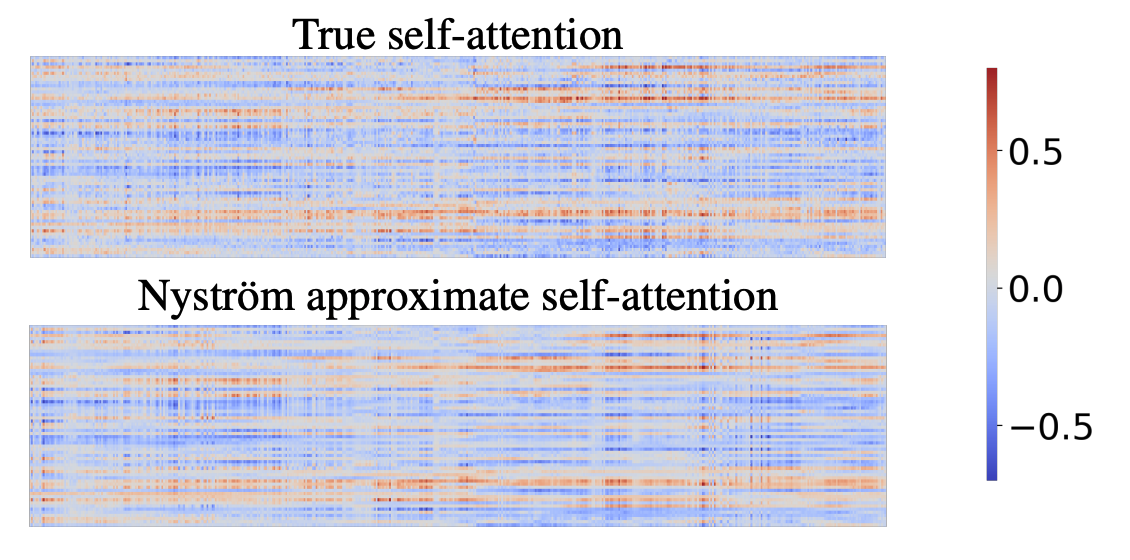
\includegraphics[width=0.5\textwidth]{nystrom-approximation.png}
\caption{\label{fig:nystrom-approximation}Illustration of Nystrom approximation vs pure self-attention. They are not identical but similar.}
\end{figure}

\section{Results}

\subsection{Computational complexity}

This section analyses the efficiency advantage of attention approaches considered in this research over dot-product attention in time (CC) \ref{fig:comutation-time} and memory (MC) \ref{tab:mem-complexity} complexities. 
To measure computational complexity, we measure the inference time that it takes to compute values on NVIDIA GPU T4 for input data $ X \in R^{ batch\_size \times num\_head \times n \times d }$, where $\textbf{batch size}=32$, $\textbf{number of heads}=4$, sequence length $\textbf{n} \in \{128, 256, 512, 768, 1024, 2048\}$ and features dimension size $\textbf{d} \in \{32, 64\}$.
Typically sequence length is defined as image pixel size, and equals 1024 for image 32x32.


\begin{figure*}[!h]
	\centering
	\begin{subfigure}[t]{0.5\textwidth}
		\centering
		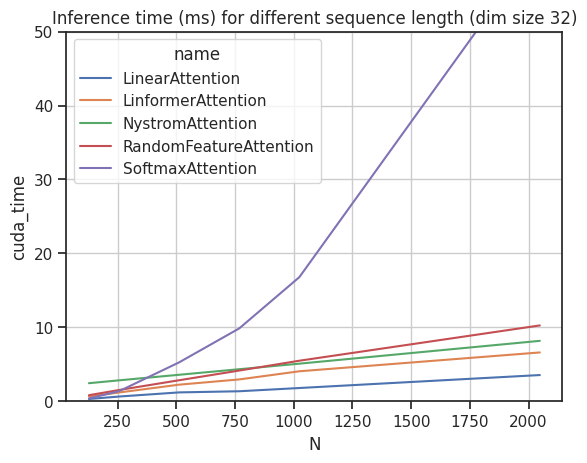
\includegraphics[scale=0.5]{speed_cuda_32.png}
		\caption{N=32} \label{comutation-time-32}
	\end{subfigure}\hfill
	\centering
	\begin{subfigure}[t]{0.5\textwidth}
		\centering
		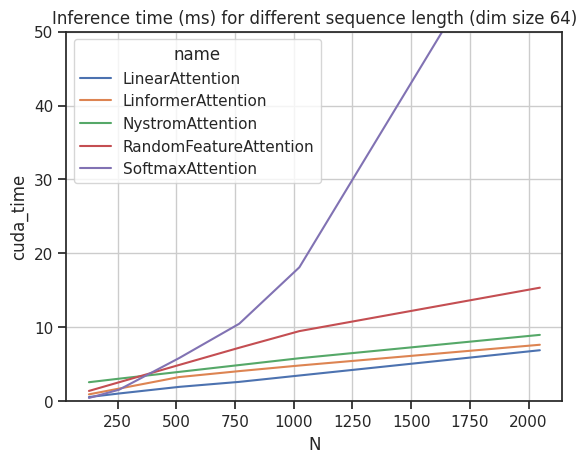
\includegraphics[scale=0.5]{speed_cuda_64.png}
		\caption{N=64} \label{comutation-time-64}
	\end{subfigure}\hfill

	\caption{Computation time on GPU in ms.}
	\label{fig:comutation-time}
\end{figure*}


\begin{table}
\centering
\begin{tabular}{l|l|l}
Method & Computational & Memory & \\\hline
Dot-product (softmax) attention & $O(d^2n+dn^2)$ &  $O(nd^2)$ \\
Linear attention & $O(d^2n)$ & $ O(dn+d^2) $  \\
Linformer Attention & $O(n)$ & $ O(n) $ \\
Random Feature Attention & $O(nd)$ & $O(4D + 2Dd)$ \\
Nystrom Attention & $O(n)$ & $O(n)$
\end{tabular}
\caption{\label{tab:mem-complexity}Methods complexity}
\end{table}


\subsection{Results on accuracy}

\begin{figure*}[!h]
	\centering
	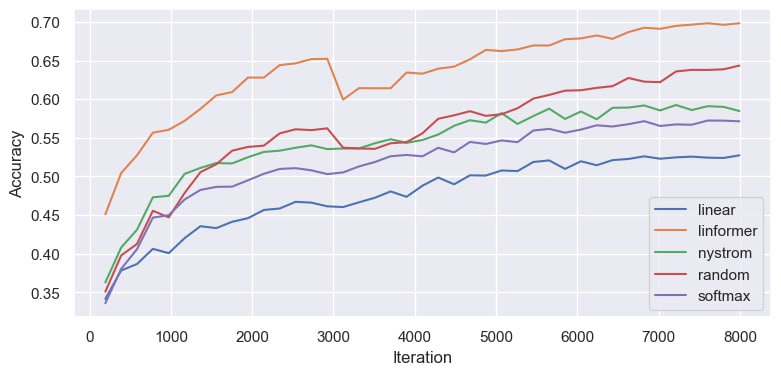
\includegraphics[scale=0.5]{attention-accuracy.jpg}
	\caption{Computation time on GPU in ms.}
	\label{fig:attention-accuracy}
\end{figure*}

We report the validation accuracy of observed models on the CIFAR-10 \cite{cifar-10}  benchmark for the 10-class image classification task. We follow the standard evaluation protocols, train the model on the training set, report the results on the validation set, and compare them to our baseline - dot-product attention. All models are trained on Tesla A100 GPUs with 50 epochs (~8k updates). The results of model accuracy depend on the iteration step and are presented in figure \ref{fig:attention-accuracy}.

\textbf{Implementation details.} Our models are trained with the cross-entropy objective. We use a batch size of 256, Adam optimizer with learning rate 5e-4, and cosine annealing scheduler, optimal parameters were estimated automatically by the Torch Lightning tool \footnote{\url{https://pytorch-lightning.readthedocs.io/en/stable/}} . Input image size is 32x32, dot-product multi-attention embedding size 256 with 8 heads. We reduced embedding size by 8 times for Linformer, and selected a fixed number of landmarks for Nystrom attention to 64.
 Please find more details on the project github \footnote{\url{https://github.com/fox-rudie/la-final-project-DS-at-UCU/tree/dev}}.



\section{Conclusions}

We investigated several methods of dot-product attention mechanism optimization in this approach using linear algebra matrix transformation techniques. It was empirically shown, that the linear attention approach has smaller computational complexity (execution speed) compared to observed methods. The Linformer attention mechanism showed the best classification accuracy compared to other observer models with similar hyper-parameters sets. Our code and setup are available at  \url{https://github.com/fox-rudie/la-final-project-DS-at-UCU/tree/dev}.


\begin{thebibliography}{unsrt}

\bibitem{self-attention-explained}
Adaloglou, N. (2021, March 25). Why multi-head self attention works: Math, intuitions and 10+1 hidden insights. AI Summer. Retrieved March 4, 2023, from https://theaisummer.com/self-attention/ 

\bibitem{linear-attention-transformer}
Katharopoulos, A., Vyas, A., Pappas, N., & Fleuret, F. (2020). Transformers are RNNs: Fast Autoregressive Transformers with Linear Attention. ArXiv. https://doi.org/10.48550/arXiv.2006.16236

\bibitem{efficient-linear-attention}
Shen, Z., Zhang, M., Zhao, H., Yi, S., & Li, H. (2018). Efficient Attention: Attention with Linear Complexities. ArXiv. https://doi.org/10.48550/arXiv.1812.01243

\bibitem{linformer}
Wang, S., Li, B. Z., Khabsa, M., Fang, H., & Ma, H. (2020). Linformer: Self-Attention with Linear Complexity. ArXiv. https://doi.org/10.48550/arXiv.2006.04768

\bibitem{jonson-lindenstrauss}
Ghojogh, B., Ghodsi, A., Karray, F., & Crowley, M. (2021). Johnson-Lindenstrauss Lemma, Linear and Nonlinear Random Projections, Random Fourier Features, and Random Kitchen Sinks: Tutorial and Survey. ArXiv. https://doi.org/10.48550/arXiv.2108.04172

\bibitem{random_feature_attention}
Peng, H., Pappas, N., Yogatama, D., Schwartz, R., Smith, N. A., & Kong, L. (2021). Random Feature Attention. ArXiv. https://doi.org/10.48550/arXiv.2103.02143

\bibitem{Rahimi_2007}
Ali Rahimi and Benjamin Recht. 2007. Random features for large-scale kernel machines. In Proceedings of the 20th International Conference on Neural Information Processing Systems (NIPS'07). Curran Associates Inc., Red Hook, NY, USA, 1177–1184.

\bibitem{orthogonal_random_features}
Yu, F. X., Suresh, A. T., Choromanski, K., & Kumar, S. (2016). Orthogonal Random Features. ArXiv. https://doi.org/10.48550/arXiv.1610.09072

\bibitem{nystrom_attention_paper}
Yunyang Xiong, Zhanpeng Zeng, Rudrasis Chakraborty, Mingxing Tan, Glenn Fung, Yin Li and Vikas Singh.
\newblock Nyströmformer: A Nyström-Based Algorithm for Approximating Self-Attention, 2021;
\newblock arXiv:2102.03902.

\bibitem{cifar-10}
Alex Krizhevsky. Learning multiple layers of features from tiny images. Technical report, 2009.

\bibitem{pseudoiverse}
Razavi, M. K.; Kerayechian, A.; Gachpazan, M.; and Shateyi, S.
2014. A new iterative method for finding approximate inverses of
complex matrices. In Abstract and Applied Analysis.

\end{thebibliography}


\end{document}